% ABOUTME: Test set results section of the IEEE report (issue #6).
% ABOUTME: Frozen models scored once on FD001 test engines, error analysis and published comparison.
\section{Test Set Results}
\label{sec:results}

\subsection{Protocol}
Every hyperparameter and the choice of selected model were fixed by cross
validation (Section~\ref{sec:models}) before the test set was opened. Each
configuration is refitted on all 100 training engines with RUL capped at
125 cycles, and the feature statistics (regime normalisation and the health
index) are fitted on the training engines and applied unchanged to the test
engines. Features are computed over each test engine's full observed
history, and the model predicts once per engine at its last observed cycle
(Section~\ref{sec:evaluation}). Predictions are scored against the true,
uncapped RUL. All numbers in this section are taken from
\texttt{results/test\_metrics.csv}.

\begin{table*}[t]
\centering
\caption{Test results on the 100 FD001 test engines, scored against the
true RUL. Late stage is true RUL $\le 50$ (33 engines), early stage is
true RUL $> 50$ (67 engines). XGBoost on engineered features was selected
by cross validation before the test set was used.}
\label{tab:test-results}
\begin{tabular}{llrrrrrr}
\hline
Model & Features & RMSE & MAE & Score $S$ & Early RMSE & Late RMSE & Late MAE \\
\hline
Mean baseline     & --         & 43.07 & 35.90 & 33629 & 27.30 & 64.09 & 62.68 \\
Linear regression & raw        & 22.54 & 17.73 & 1291  & 21.93 & 23.72 & 19.83 \\
Elastic Net       & raw        & 22.57 & 17.77 & 1296  & 21.93 & 23.82 & 19.95 \\
Random Forest     & raw        & 17.77 & 13.21 & 534   & 19.42 & 13.83 & 8.90 \\
XGBoost           & raw        & 17.58 & 13.01 & 539   & 19.39 & 13.17 & 8.22 \\
Linear regression & engineered & 18.23 & 14.10 & 519   & 19.69 & 14.85 & 12.68 \\
Elastic Net       & engineered & 18.27 & 14.11 & 522   & 19.75 & 14.83 & 12.64 \\
Random Forest     & engineered & 15.23 & 11.33 & 344   & 17.88 & 7.34  & 5.06 \\
XGBoost (selected) & engineered & 15.36 & 11.26 & 389  & 18.11 & 7.03  & 5.25 \\
\hline
\end{tabular}
\end{table*}

\subsection{Overall results}
Table~\ref{tab:test-results} gives the results. The selected XGBoost model
reaches an RMSE of 15.36 cycles, an MAE of 11.26 and a score of 389. In the
late stage, where maintenance is scheduled, its RMSE is 7.03 cycles.
Random Forest is slightly better on the test set (RMSE 15.23, score 344),
although cross validation had ranked XGBoost first (13.99 against 14.42).
We keep the selection, because changing it after seeing test results would
make the test set a second validation set and bias the reported error
downwards.

With only 100 test engines, a gap this small may be sampling noise. A
paired bootstrap, resampling the 100 engines 10{,}000 times and scoring
both models on the same resample, gives a 95\% interval of $-1.3$ to
$+1.1$ cycles for the RMSE of Random Forest minus XGBoost, so the two
ensembles cannot be separated. The intervals for XGBoost minus Elastic Net
($-4.8$ to $-1.0$) and for XGBoost on engineered minus raw features
($-4.4$ to $-0.2$) exclude zero. The two conclusions of cross validation
therefore hold on unseen engines: tree ensembles beat the linear models,
and the engineered features improve every model, most of all in the late
stage, where XGBoost's RMSE falls from 13.17 to 7.03.

\begin{figure*}[t]
  \centering
  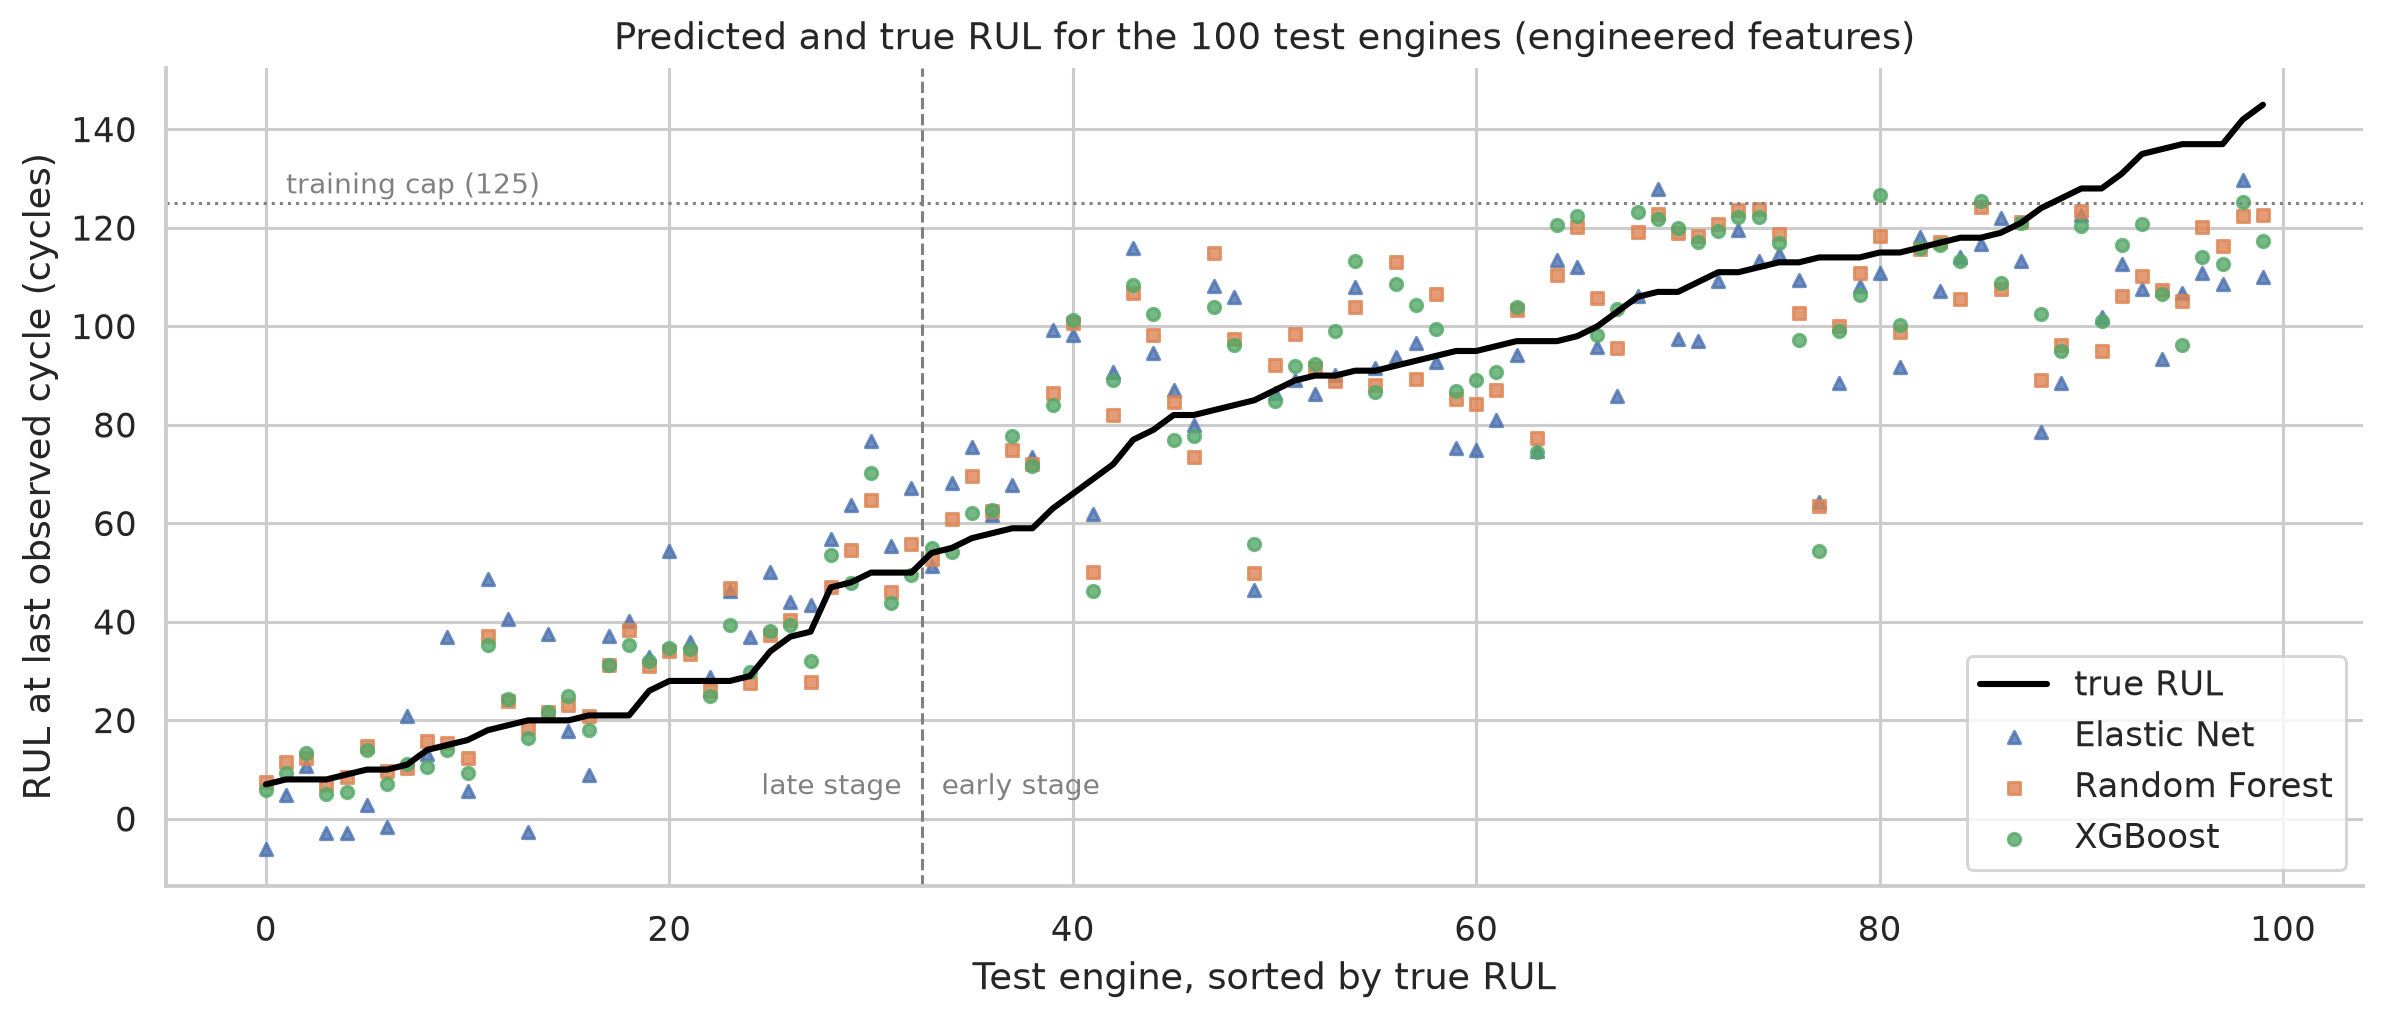
\includegraphics[width=\textwidth]{../figures/results_pred_vs_true.png}
  \caption{Predicted and true RUL at the last observed cycle of each test
  engine, sorted by true RUL. The dashed line separates the late stage
  (left) from the early stage; the dotted line is the training cap.}
  \label{fig:results-pred}
\end{figure*}

\subsection{Where the errors are}
Fig.~\ref{fig:results-pred} and Fig.~\ref{fig:results-buckets} show how
the error depends on the true RUL. For both tree ensembles the error is
smallest close to failure, with RMSE of about 7 cycles for true RUL of at
most 25 and about 8 between 26 and 50. It rises to between 16 and 17.5
cycles from 51 to 125. Elastic Net is close to the ensembles far from
failure but about twice as inaccurate in the late stage, which is where the
trees gain most. Between 51 and 75 cycles all three models predict too late
(median error $+9$ to $+14$ cycles), around the point where degradation first
becomes visible in the sensors. Eleven test engines have a true RUL above
the training cap (up to 145). No model predicts much above 125, because no
training target was larger, so these engines are underestimated by 23 to
26 cycles on average, about 10 of them by construction. Underestimating brings maintenance forward, which
is the cheaper error.

\begin{figure*}[t]
  \centering
  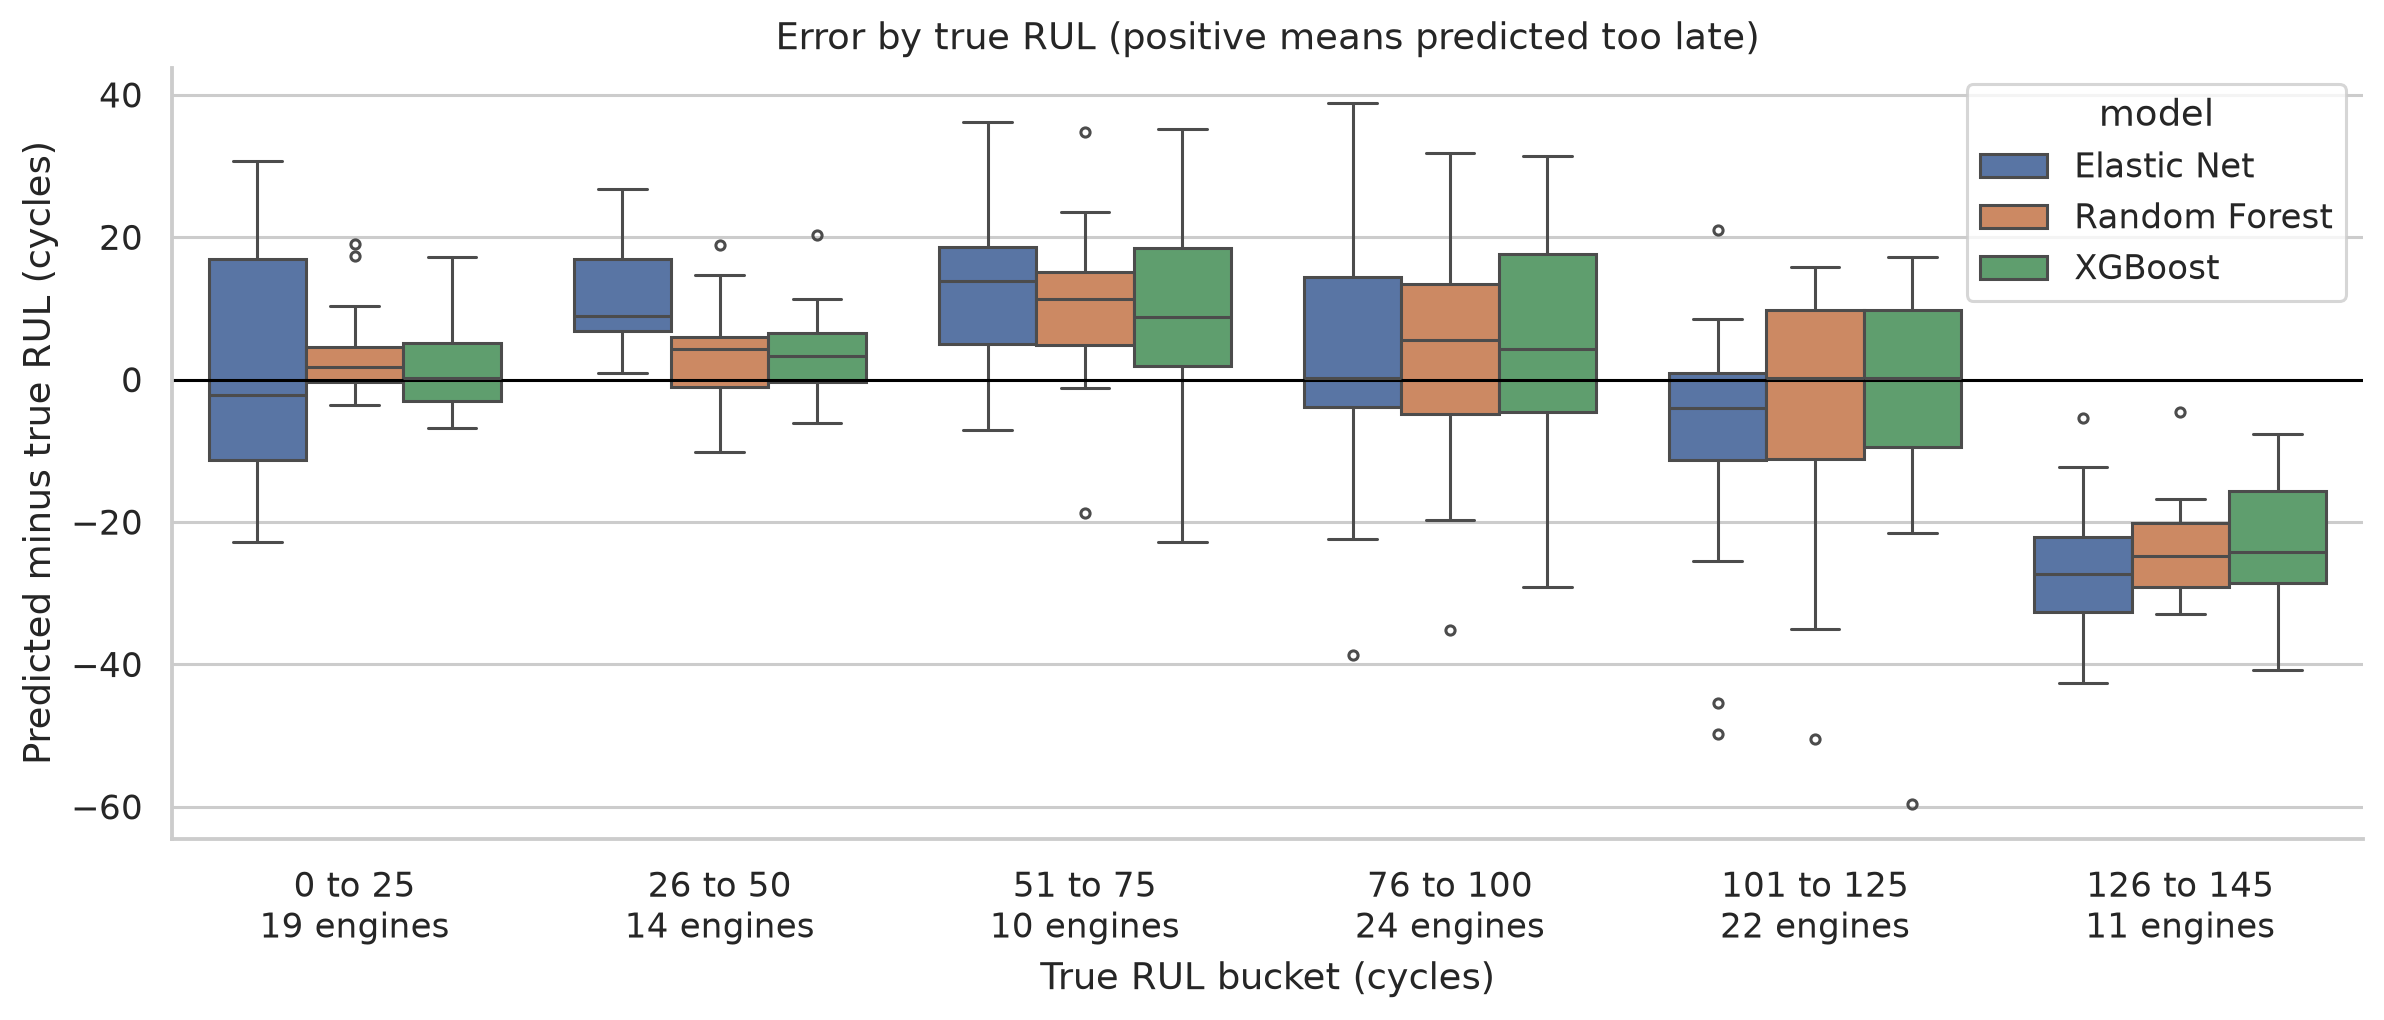
\includegraphics[width=\textwidth]{../figures/results_error_by_bucket.png}
  \caption{Prediction error (predicted minus true RUL) by true RUL bucket for
  the three tuned models on engineered features. Positive errors are late
  predictions.}
  \label{fig:results-buckets}
\end{figure*}

The residual distributions (Fig.~\ref{fig:results-residuals}) are centred
near zero, with mean errors between $-1.0$ and $+0.1$ cycles. The difference
in score between the two ensembles comes from the costly side: 6 Random
Forest predictions and 9 XGBoost predictions are more than 20 cycles late.
Because $S$ grows exponentially with lateness, these few engines account
for most of the gap between 344 and 389, even though the RMSEs are almost
equal.

\begin{figure}[t]
  \centering
  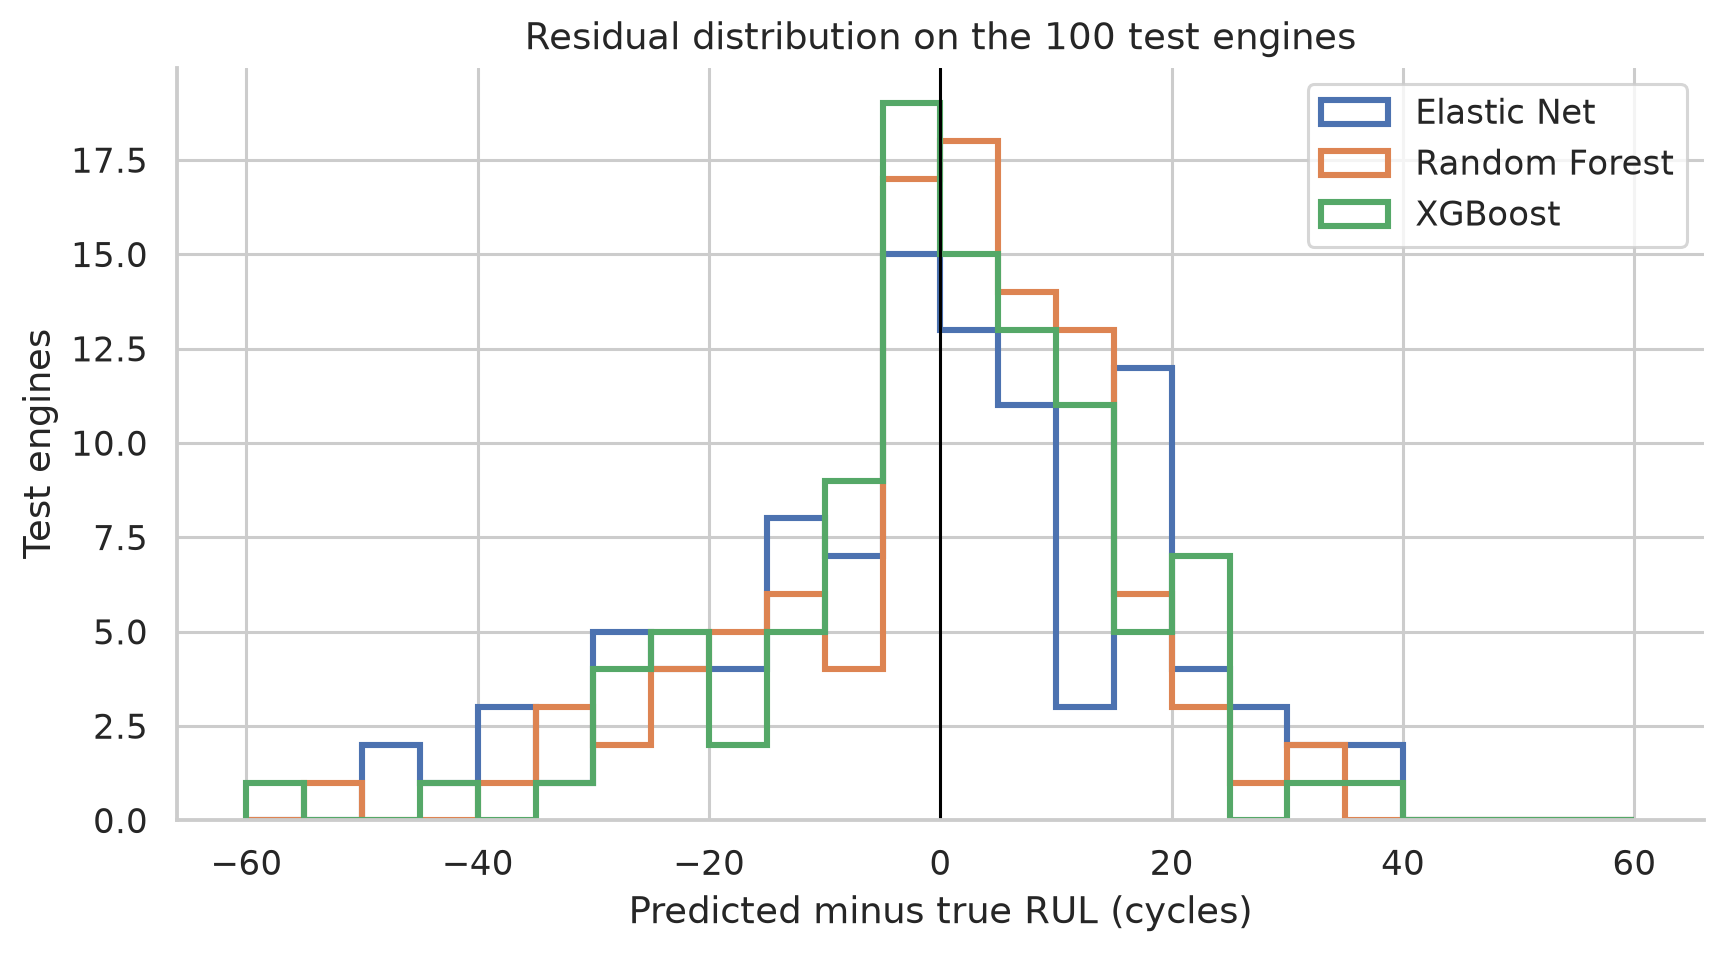
\includegraphics[width=\columnwidth]{../figures/results_residuals.png}
  \caption{Distribution of test errors for the three tuned models on
  engineered features.}
  \label{fig:results-residuals}
\end{figure}

\subsection{Comparison with published results}
Published FD001 results typically train on RUL capped at 125 and score one
prediction per test engine, as we do, but many also clip the test labels at
the cap. For a like for like comparison we rescore our models against the
test RUL clipped at 125. Table~\ref{tab:published} lists every FD001 result
with both RMSE and score collected by Ragab et al.~\cite{ragab2020attention},
except an SVM baseline (RMSE 40.72). By RMSE our Random Forest (14.02) and
XGBoost (14.08) rank fifth and sixth. They improve on the published Random
Forest (17.91) and gradient boosting (15.67) of Zhang et
al.~\cite{zhang2017modbne} and on six deep models, from CNN-LSTM (14.40) to
the 2D CNN of Babu et al.~\cite{babu2016cnn} (18.45). Our own raw feature
models score 16.58 and 16.37 against the same labels, so in our setting most
of the improvement comes from the engineered features rather than the
learner.

Four published deep models are more accurate: the 1D CNN of Li et
al.~\cite{li2018dcnn} (12.61), the attention model of Ragab et
al.~\cite{ragab2020attention} (12.63), HDNN (13.02) and BLCNN (13.18), between
0.8 and 1.4 cycles of RMSE ahead of our Random Forest. On the score $S$ our
position is weaker: six published models score lower than our Random
Forest (310), including BiLSTM-ED and CNN-LSTM, whose RMSE is higher than
ours but whose predictions are less often badly late. The models ahead of
ours learn features from windows of the raw sensor sequence; phase 2 of this
project tests sequence models of this kind. Published protocols differ in
details that are not always reported, such as window length, so differences
of a fraction of a cycle should not be over read.

\begin{table}[t]
\centering
\caption{FD001 test results against labels clipped at 125; ours use the
engineered features. Published values as collected in
\cite{ragab2020attention}, Table III, which cites the original papers for
rows without a reference here.}
\label{tab:published}
\begin{tabular}{lrr}
\hline
Method & RMSE & Score $S$ \\
\hline
1D CNN \cite{li2018dcnn}             & 12.61 & 274 \\
ATS2S \cite{ragab2020attention}      & 12.63 & 243 \\
HDNN                                 & 13.02 & 245 \\
BLCNN                                & 13.18 & 302 \\
Random Forest (ours)                 & 14.02 & 310 \\
XGBoost (ours)                       & 14.08 & 347 \\
CNN-LSTM                             & 14.40 & 290 \\
BiLSTM-ED                            & 14.74 & 273 \\
LSTMBS                               & 14.89 & 481 \\
MODBNE \cite{zhang2017modbne}        & 15.04 & 334 \\
Gradient boosting \cite{zhang2017modbne} & 15.67 & 474 \\
Deep LSTM \cite{zheng2017lstm}       & 16.14 & 338 \\
Elastic Net (ours)                   & 17.01 & 469 \\
Random Forest \cite{zhang2017modbne} & 17.91 & 480 \\
2D CNN \cite{babu2016cnn}            & 18.45 & 1287 \\
\hline
\end{tabular}
\end{table}
